\documentclass{standalone}
\usepackage{tikz}
\usetikzlibrary{arrows.meta}
\tikzset{label/.style = {inner sep=1pt, fill=white}}
%\tikzset{nd/.style={circle, inner sep=0pt}}
\tikzset{nd/.style={inner sep=1pt}}
\tikzset{>=Latex}
\tikzset{arc/.style = {->, semithick, >=Latex}}
\begin{document}
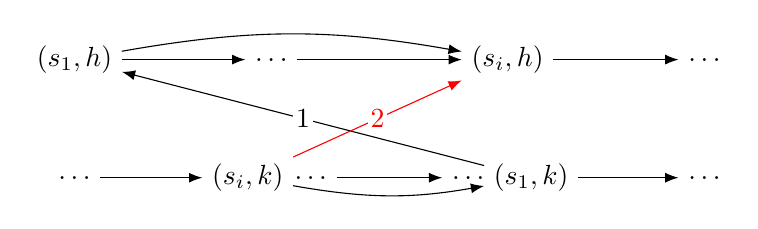
\begin{tikzpicture}
    
    \node (s1) at (0,1.5) {$(s_1,h)$};
    \node (d1) at (2.5,1.5) {$\dots$};
    %\node (sw) at (2.5,1.5) {$(s_\omega,j)$};
    \node (d2) at (5.5,1.5) {$(s_i,h)$};
    %\node (d3) at (5,1.5) {$\dots$};
    %\node (sa) at (5.5,1.5) {$s_\alpha$};
    %\node (d4) at (6,1.5) {$\dots$};
    \node (sn) at (8,1.5) {$\dots$};
    
    \node (s1b) at (0,0) {$\dots$};
    %\node (d1b) at (2,0) {$\dots$};
    \node (swb) at (2.2,0) {$(s_i,k)$};
    \node (d2b) at (3,0) {$\dots$};
    \node (d3b) at (5,0) {$\dots$};
    \node (sab) at (5.8,0) {$(s_1,k)$};
    %\node (d4b) at (6,0) {$\dots$};
    \node (snb) at (8,0) {$\dots$};
    
    \draw[->] (s1) to (d1);
    \draw[->] (d1) to (d2);
    \draw[->] (d2) to (sn);
    
    \draw[->] (s1b) to (swb);
    \draw[->] (d2b) to (d3b);
    \draw[->] (sab) to (snb);
    
    \draw[->] (sab) to node[label=above] {1} (s1);
    \draw[->] (s1) to [out = 10, in = 170] (d2);
    \draw[->] (swb) to [out = -10, in = -170] (sab);

    \draw[->,red] (swb) to node[label=above] {2} (d2);
 \end{tikzpicture}
\end{document}